\documentclass[../main.tex]{subfiles}

\begin{document}

\section*{東大理科数学 2005年}

\subsection*{第1問}

\noindent
\textbf{[解]} 題意を M.I. で示す. $n=1$ の時
\[
  f'(x) = \frac{1 - \log x}{x^2}
\]
だから $a_1 = 1, b_1 = -1$ とすれば良い. $n=k$ での成立を仮定する.
\begin{align*}
  f^{(k+1)}(x) &= \frac{b_k \cdot x^k - (k+1) \cdot x^k (a_k + b_k \log x)}{(x^{k+1})^2} \\
  &= \frac{(b_k - (k+1) a_k) + (-(k+1) b_k) \log x}{x^{k+2}}
\end{align*}
だから
\[
  \begin{cases}
    a_{k+1} = -(k+1) a_k + b_k \\
    b_{k+1} = -(k+1) b_k
  \end{cases}
\]
とすれば $n=k+1$ でも成立.

\bigskip

\noindent
以上より示された. 同漸化式は
\[
  \begin{cases}
    a_{n+1} = -(n+1) a_n + b_n &, a_1 = 1 \\
    b_{n+1} = -(n+1) b_n &, b_1 = -1
  \end{cases}
\]

\bigskip

\noindent
(2) (1)から, $b_n = (-1)^n n!$ であるから,
\[
  a_{n+1} = -(n+1) a_n + (-1)^n \cdot n! \quad \cdots \textcircled{1}
\]
$c_n = \frac{a_n}{(-1)^n n!}$ とおいて ($c_1 = -1$), \textcircled{1}の両辺を $(-1)^{n+1} (n+1)!$ で割ると
\[
  c_{n+1} = c_n + \frac{1}{-(n+1)}
\]
だから, 階差数列より $n \ge 2$ の時
\begin{align*}
  c_n &= c_1 + \sum_{k=2}^n \frac{1}{-k} \\
  &= -h_n
\end{align*}
$n=1$ でもこれは成立するから
\[
  a_n = (-1)^{n+1} \cdot n! \cdot h_n
\]
である.

\newpage

\subsection*{第2問}

\noindent
\textbf{[解]} $w = z^2 - 2z$ から $z = 1 \pm \sqrt{1+w}$ であるから,
\[
  |z| \le \frac{5}{4} \iff |1 \pm \sqrt{1+w}| \le \frac{5}{4}
\]
だから, $\sqrt{1+w}$ の存在領域は右図斜線部 (境界含む). $\sqrt{1+w} = x + yi \; (x,y \in \mathbb{R})$ とおくと,
$w = (x^2 - y^2 - 1) + 2xy i$ で,
\[
  |w|^2 = (x^2 - y^2 - 1)^2 + 4x^2 y^2
\]
これは $x \to -x, y \to -y$ について対称だから, $x \ge 0, y \ge 0$ で考えれば良い. この時,
\[
  0 \le x \le \frac{1}{4}, \quad 0 \le y \le \sqrt{\left(\frac{5}{4}\right)^2 - (x+1)^2} \quad \cdots \textcircled{1}
\]
であり,
\[
  |w|^2 = [ y^2 + (x+1)^2 ]^2 - 4x^2
\]
\textcircled{1}から $x$ を固定した時, $|w|^2$ は $y = \sqrt{\left(\frac{5}{4}\right)^2 - (x+1)^2}$ で最大で (軸が $y>0$ にある)
\begin{align*}
  \max |w|^2 &= \left\{ 2x^2 + 2x - \frac{15}{16} \right\}^2 + 4x^2 \left\{ \frac{25}{16} - (x+1)^2 \right\} \\
  &= -\frac{25}{4} x + \left(\frac{5}{4}\right)^2
\end{align*}
これは $x=0$ で $\max |w| = \frac{25}{16}$ をとる. したがって, $|w|$ が最大の時, $x=0, y=\frac{3}{4}$ でこの時
\[
  w = -\frac{25}{16}
\]
である.

\begin{center}
  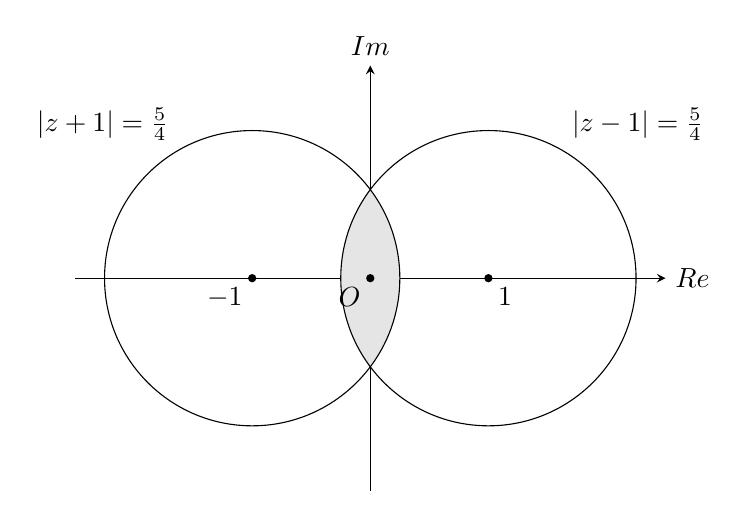
\begin{tikzpicture}[scale=1.5, >=stealth]
    \draw[->] (-2.5,0) -- (2.5,0) node[right] {$\text{Re}$};
    \draw[->] (0,-1.8) -- (0,1.8) node[above] {$\text{Im}$};
    \begin{scope}
      \clip (-1,0) circle (1.25);
      \fill[gray!20] (1,0) circle (1.25);
    \end{scope}
    \draw (-1,0) circle (1.25);
    \draw (1,0) circle (1.25);
    \node[above left] at ({-1 + 1.25*cos(120)}, {1.25*sin(120)}) {$|z+1|=\frac{5}{4}$};
    \node[above right] at ({1 + 1.25*cos(60)}, {1.25*sin(60)}) {$|z-1|=\frac{5}{4}$};
    \fill (-1,0) circle (1pt) node[below left] {$-1$};
    \fill (1,0) circle (1pt) node[below right] {$1$};
    \fill (0,0) circle (1pt) node[below left] {$O$};
  \end{tikzpicture}
\end{center}

\bigskip

\noindent
\textbf{[解2]} $z$ の2次方程式 $z^2 - 2z - w = 0$ の2解を $z_1, z_2$ とする.
\[
  \begin{cases}
    z_1 + z_2 = 2 \\
    z_1 z_2 = -w
  \end{cases} \quad \cdots \textcircled{1}
\]
ならば $|z_1|, |z_2| \le \frac{5}{4}$ となるような $w$ をかんがえれば良い.
\[
  |w| = |-z_1 z_2| = |z_1| |z_2| \le \frac{25}{16}
\]
等号成立する時, $z_1, z_2 = 1 \pm \frac{3}{4}i$ で十分. この時 $w = -\frac{25}{16}$. \hfill $\qed$

\bigskip

\subsection*{第3問}

\noindent
{\bf [解]}
(1) $f(x)=\dfrac12x\{1+e^{-2(x-1)}\}$である．
\begin{align*}
  f'(x)&=\frac12\left[(1+e^{-2(x-1)})+x(-2)e^{-2(x-1)}\right]\\
  &=\frac12\left[1+(1-2x)e^{-2(x-1)}\right]
\end{align*}
である．$\dfrac12<x$の時，$(1-2x)e^{-2(x-1)}<0$だから，$f'(x)<\dfrac12\quad\cdots①$である．
\begin{align*}
  f''(x)&=\frac12e^{-2(x-1)}\left[-2+(1-2x)(-2)\right]\\
  &=-e^{-2(x-1)}(2-2x)
\end{align*}
から下表を得る．
\begin{center}
  \begin{tabular}{c|ccccc}
    $x$ & $\frac12$ & $\cdots$ & $1$ & $\cdots$ & $\infty$\\
    \hline
    $f''$ & & $-$ & $0$ & $+$ & \\
    $f'$ & & $\searrow$ & $0$ & $\nearrow$ & \\
  \end{tabular}
\end{center}
したがって，$\dfrac12<x$の時，$0\le f'(x)\quad\cdots②$である．①②から示された．$\blacksquare$

(2) $f(1)=1$だから，
\begin{align*}
  x_{n+1}-1=f(x_n)-f(1)\quad\cdots③
\end{align*}

$x_n=1$なる$n$がある時，③から$n\le m$なる任意の$m$に対し，$f(x_m)=1$だから，$x_n\to1\ (n\to\infty)$である．

以下，すべての$n$で$x_n\ne1$の場合を考える．$(1)$の表から$x>\dfrac12$の時$f(x)$は単調増加で$f\left(\dfrac12\right)=\dfrac14(1+e)>\dfrac12$だから，$x>\dfrac12\implies f(x)>\dfrac12$である．$x_0>\dfrac12$だから，帰納的に任意の$n$に対し$x_n>\dfrac12$である．

このことに注意すると，平均値の定理から（$\because f(x)$が微分可能である），
\begin{align*}
  f(x_n)-f(1)=f'(c)(x_n-1)\quad\left(c\text{は}\frac12<c\text{，}1\text{と}x_n\text{の間}\right)
\end{align*}
なる$c$がある．③から，
\begin{align*}
  |x_{n+1}-1|=|f'(c)||x_n-1|<\frac12|x_n-1|\quad(\because(1))
\end{align*}

くり返し用いて，
\begin{align*}
  |x_n-1|<\left(\frac12\right)^n|x_0-1|\longrightarrow0\quad(n\to\infty)
\end{align*}

はさみうちから
\begin{align*}
  x_n\longrightarrow1\quad(n\to\infty)
\end{align*}

\bigskip

\subsection*{第5問}

\noindent
{\bf [解]}
$k=a+b$とおく．甲が勝つのは，以下の条件が全て満たされる時である．
\begin{align*}
  k&\le N\quad\cdots①\\
  k&\ge c\quad\cdots②\\
  k&<c+d\le N\text{とならない}\quad\cdots③
\end{align*}

まず③について，①②に注意すると，$c=1,2,\ldots,k$の$k$通りであり，各$c$（$1\le c\le k$）に対し，③をみたす（すなわち$c+d\le k$または$c+d>N$となる）$d\in\{1,\ldots,N\}$の個数を数える．$c+d\le k\iff d\le k-c$から，この範囲の$d$は$1,\ldots,k-c$の$k-c$個．$c+d>N\iff d>N-c$から，この範囲の$d$は$N-c+1,\ldots,N$の$c$個．$k\le N$から$k-c\le N-c$なので，これら2つの範囲は重ならず，あわせて$(k-c)+c=k$個である．したがって，$d$は各$c$に対して$k$通りであり，$c,d$の定め方は，$k$ひとつに対して$k^2$通りである．$\cdots④$

(1) $k=a$の時，全事象は$N^2$通りだから，
\begin{align*}
  P=\left(\frac aN\right)^2
\end{align*}

(2) $k=a+1,\ldots,N$の時（$a\ne N$の場合も含め空和で対応），④から，甲が勝つ場合の数は
\begin{align*}
  \sum_{k=a+1}^Nk^2=\frac16\left[N(N+1)(2N+1)-a(a+1)(2a+1)\right]
\end{align*}
であり，$a=N$の時の場合の数$0$にも対応している．全事象は$N^3$通りだから，
\begin{align*}
  P=\frac1{6N^3}\left[N(N+1)(2N+1)-a(a+1)(2a+1)\right]
\end{align*}

\end{document}
